\chapter{IT Trends}
\section{Grundbegriffe zu Trends}
\subsection{Begriffsdefinition}
Der Begriff \textit{trend} stammt aus dem Englischen \textit{to trend}, was so viel bedetet wie \textit{in bestimmte  Richtung verlaufen}. Generell ist es eine Veränderung in der Gesellschaft / Wirtschaft oder Technik, welche eine neue Bewegung oder Richtung auslöst.
\subsection{Trend als Extrapolation}
Ein Trend kann man gut beobachten, aber schlecht messen. Man nimmt dazu bereits bekannte Daten, analysiert die und versucht, eine Aussage über den Verlauf in der Zukunft zu treffen. Typischerweise kann man den Trend selbst nicht beeinflussen. Dabei trifft man auch auf das Problem der sich selbst erfüllenden Prophezeiung - wenn man sagt, dass Firma X in den nächsten Jahren sehr stark sein wird, so ist das Vertrauen in die Firma grösser und die Wahrscheinlichkeit höher, dass sie tatsächlich sehr stark sein wird.
\begin{figure}
\centering
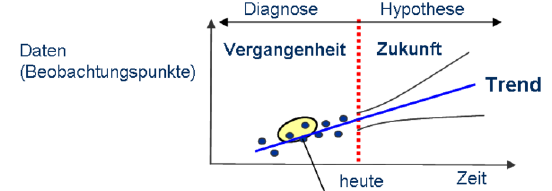
\includegraphics[width=0.7\linewidth]{fig/trend}
\caption{Anatomie eines Trends}
\label{fig:trend}
\end{figure}
\subsection{Quellen}
Trends werden z.B. von Business Analysten und Beratungsfirmen, aber auch von den Technologie Unternehmen selbst publiziert. Die Technologie Unternehmen publizieren diese, da sie ihre Innovationskraft demonstrieren möchten, verwenden es also als \textbf{Marketinginstrument}. Die Business Analysten  / Beratungsfirmen verdienen damit ihre Brötchen!
\subsection{Faktoren die zu Trends führen}
Oder einfach Faktoren, welche unsere Zukunft mitbestimmen. Diese sind extrem vielfältig, und haben 5 Kernpunkte;
\begin{enumerate}
	\item Gesellschaft
	\item Biosphäre
	\item Technologie
	\item Politik
	\item Wirtschaft
\end{enumerate}
Diese Kernpunkte beeinflussen sich alle gegenseitig.
\subsection{Trenddarstellungen}
Es gibt verschiedene Wege, wie man einen aktuellen / vergangenen Trend darstellen kann. Diese sind nachfolgend vorgestellt.
\subsubsection{Hypekurve}
\begin{figure}
\centering
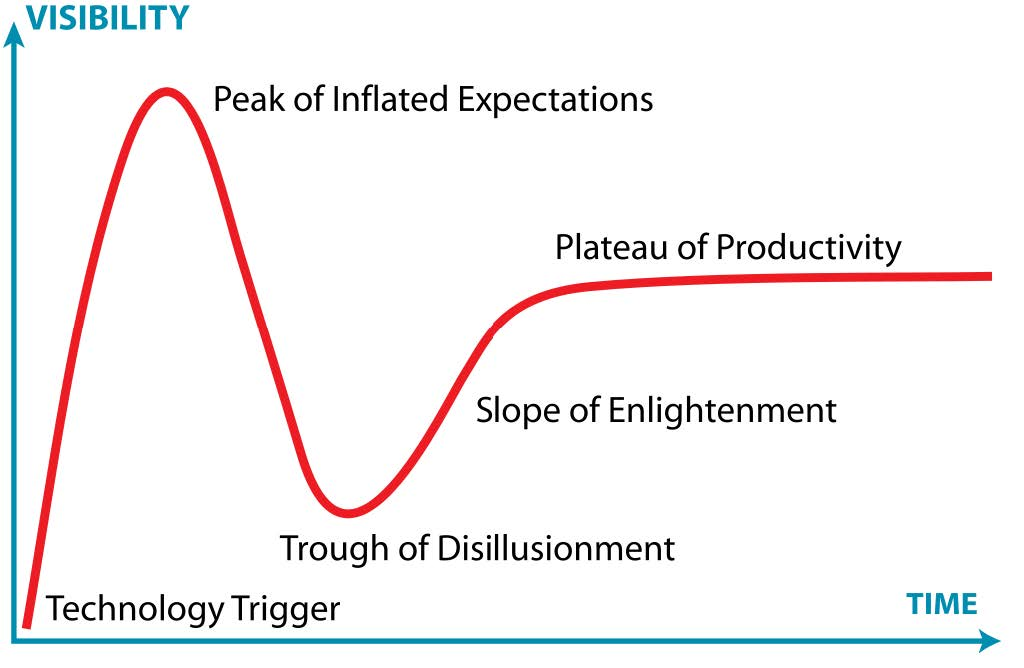
\includegraphics[width=0.7\linewidth]{fig/hype_kurve}
\caption{Die Hypekurve}
\label{fig:hype_kurve}
\end{figure}
Die Hypekurve beschreibt folgendes Phänomen: Am Anfang ist die Technologie noch unbekannt, deswegen am Boden. Danach wird die Technologie entdeckt und überall gross in den Medien präsentiert, wobei natürlich grosse Erwartungen in die Technologie gesteckt werden. Danach sinkt das Interesse relativ schnell, da die Erwartungen nicht erfüllt werden konnten. Später, wenn das \textit{wahre} Potenzial der Technologie erkannt wurde, steigt die Visibliät nochmals und bleibt stabil. \\
Der Nachteil an dieser Darstellung ist, dass sie gar keine Vorhersagekraft besitzt, sondern nur den aktuellen Stand kommentiert. Zudem entbehrt sie jeglichen wissenschaftlichen Grundlagen und missachtet den Fakt, dass ein Top oder Flop nicht nur von der Technologie abhängig ist, und es durchaus möglich ist, dass eine Technologie auch einfach verschwindet, ohne je das \textit{Plateau of Productivity} erreicht zu haben.
\subsubsection{Trendliste}
Eine einfache Liste, was denn im Moment am Aufstreben ist. Lässt sich über die Jahre vergleichen - war dieser Trend tatsächlich richtig?
\subsubsection{Trendwellen}
Trends treten in Wellenform auf - leider verstehe ich das nicht und im Internet tritt diese Grafik extrem selten auf...
Reviewer - Entscheide ob du obs rein gehört oder raus muss.
\begin{figure}
\centering
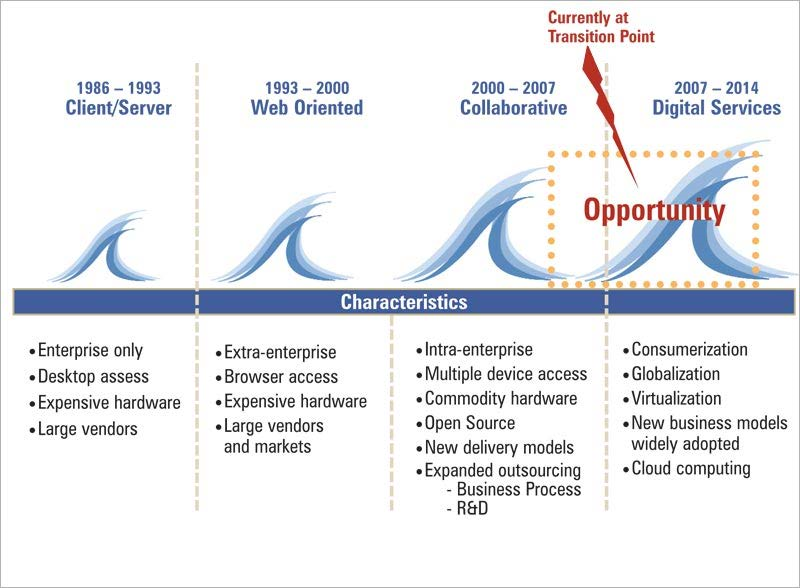
\includegraphics[width=0.7\linewidth]{fig/waves}
\caption{}
\label{fig:waves}
\end{figure}

\section{Trendkritik, Spekulationen, Kontroversen}
\subsection{Hardware vs Fähigkeit}
Nur weil man eine Videokamera und einen PC hat, heisst das noch lange nicht dass man damit einen Kinofilm herstellen kann. Das heisst, dass wir heute zwar aus der Perspektive der Rechenleistung die Möglichkeit haben, einen Menschen zu simulieren, praktisch aber die Fähigkeit dazu (noch?) nicht haben.
\subsection{Wie gut ist eine Trendanalyse?}
Dies kann man anhand folgender Faktoren bewerten:
\begin{enumerate}
	\item Qualität der Daten (z.B. Umfang der Stichproben)
	\item Unabhängigkeit/Interessen der Analysenhersteller
	\item Wie weit voraus gehen die Prognosen?
	\item Art der Aussagen in der Analyse
	\item Sind andere derselben Meinungen? Gibt es andere, zusammenhängende Trends?
\end{enumerate}

\section{Vergangene und aktuelle Trends}
\subsection{Vergangene Trends}
\begin{enumerate}
	\item \textbf{Moore's Law} \\
		Anzahl der Transistoren pro Fläche verdoppelt sich alle 12 Monate (oder 18 oder 24).
	\item \textbf{Smartphones}
	\item \textbf{Soziale Netzwerke}
	\item \textbf{VoIP}
	\item \textbf{LEDs}
	\item \textbf{...}
\end{enumerate}
Es zeigt sich, dass auch Gartner (deren Kerngeschäft es ist, Aussagen über Trends zu treffen), oftmals nicht ganz so richtig liegen wie sie das gerne hätten, auch wenn es nur um Prognosen für die nächsten 2/3 Jahre geht. So sagten sie beispielweise, dass 2015 25\% der Arbeitsstunden beim Betrieb von IT Services durch den Einsatz von Automationstools eingespart werden.
\subsection{Aktuelle Trends (2015)}
\begin{enumerate}
	\item Computing Everywhere
	\item Internet of Things
	\item 3D Printing
	\item Advanced, Pervasice and Invisible Analytics
	\item Context-Rich Systems
	\item Smart Machines
	\item Cloud/Client Computing
	\item Software Defined Applications \& Infrastructure
	\item Web-Scale IT
	\item Risk-Based Security and Self-Protection
\end{enumerate}

\section{Cloud \& Big Data Trends umsetzen}
\subsection{Definition}
Jetzt hat jedes Fach eine Definition von Cloud, die hier kommt vom National Institute of Standards and Technology, also  vertrauenswürdiger als Chip Online...
\textit{A model for enabling ubiquitous, convenient, on-demand network access to a shared pool of configurable computing resources (e.g. networks, servers, storage, applications, and services) that can be rapidly provisioned and released with minimal management effort or service provider interaction.}
\subsection{Merkmale}
Auch hier...
\begin{enumerate}
	\item \textbf{Leistung nach Bedarf}
	\item \textbf{Abrechnung nach Nutzung}
	\item xyz as a Service
	\item Verteilt und mehrfach genutzt
	\item Internet Technologie basiert
\end{enumerate}
Klar, es gibt SaaS, PaaS und IaaS, kennen wir aus SSM.
\subsection{Warum Cloud?}
Ich wiederhole mich, wenn ich sage, dass sich das hier wiederholt. Tue aber ich, und das hier tut es auch. Yo dawg I heard you like repeations.
\begin{enumerate}
	\item Schnelle Reaktion auf Veränderungen
	\item Niedrigere Fixkosten \& Transparenz in den Kosten
	\item Fokus auf Kerngeschäft
	\item Weniger Know-How zum Betrieb notwendig
	\item Know-How der Anbieter zum eigenen Vorteil nutzen (Neue Technologien \& Referenzarchitekturen)
\end{enumerate}
\subsection{Warum nicht Cloud}
\begin{enumerate}
	\item Werden Standards in der Cloud beachtet? Kann ich einfach wieder weg?
	\item Wie stabil ist mein Anbieter?
	\item Habe ich die Kontrolle über meine Daten noch?
	\item Muss ich mir neue Skills aneignen, um die Cloud effektiv nutzen zu können?
	\item Wie sieht es mit der Cloud Governance aus?
\end{enumerate}
\subsection{Governance in der Cloud}
\begin{enumerate}
\item Wer im Unternehmen kauft externe Cloud Services ein?
\item Sind die Einkäufer juristische Vertreter des Unternehmens?
\item Wer prüft die Verträge?
\item Welches Recht kommt zur Anwendung bei Problemen?
\item Welches Preismodell ist gut für Ihr Unternehmen?
\item Wo sind die Daten und wie steht es um Datenschutz und Zugriff?
\item Wieviel Zeit bleibt, wenn sich ein Cloudservice ändert?
\item Wieviel Zeit haben Sie, wenn der Service verschwindet?
\item Was ist zu tun, wenn Sie den Cloudanbieter wechseln wollen? Geht es überhaupt? Wieviel wird es kosten?
\item Welche Informationswege, Entscheidungsprozesse, Eskalationsmechanismen bestehen mit dem Cloudanbieter?
\item Wie sichern Sie Transparenz?
\item Was heisst Backup in der Cloud?
\item Haben Sie den Zugriff auf alle Informationen, um Berichtspflichten und Audits erfüllen zu können?
\item Wissen Sie, welche anderen Cloudanbieter Ihr Vertragspartner involviert hat?
\item Wer haftet für Schäden?
\end{enumerate}
\subsection{Mögliche Strategie für den Wechsel in die Cloud}
DoD = Department of Defense (USA)
\begin{figure}
\centering
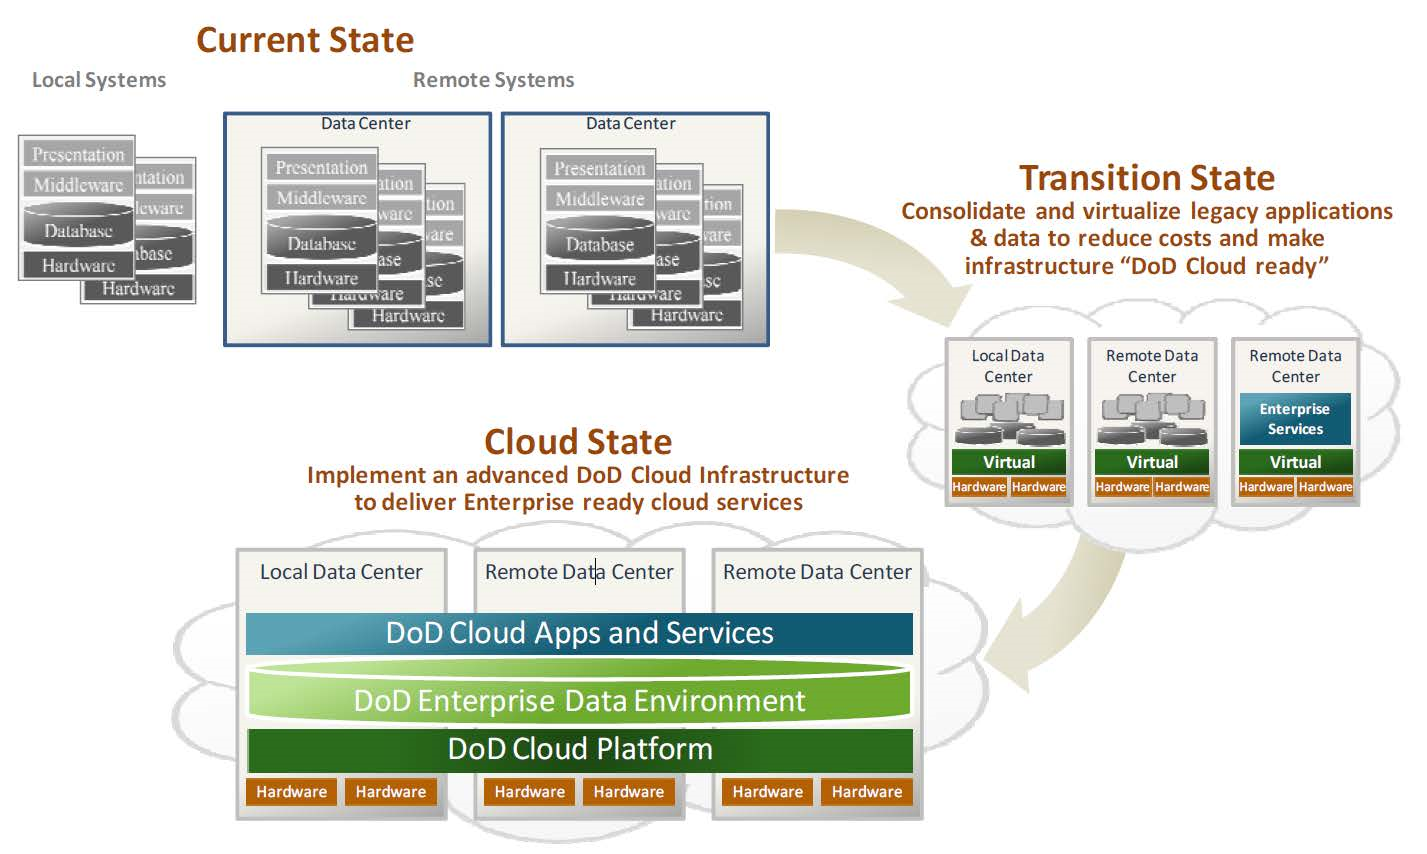
\includegraphics[width=0.7\linewidth]{fig/dod_cloud_transition}
\caption{Department of Defense Cloud Transition}
\label{fig:dod_cloud_transition}
\end{figure}
Zuerst haben wir überall unsere Applikations-Silos, mit eigener Hardware, eigenen Datenbanken \& Middleware, ... Das brechen wir im \textit{Transition State} auf, und virtualisieren die ganze Chose zuerst einmal, wobei wir auch Enterprise Services von extern implementieren. Zum Schluss haben wir eine homogene Umgebung, welche komplett in der Cloud und auf Service-Basis funktioniert.\\
Allgemein sollten bei der Implementierung von Cloud Services zuerst die SaaS-Angebote geprüft werden, und möglichst viel davon sollte daraus abgedeckt werden. Danach PaaS und zuletzt IaaS.
\subsection{Cloud Typen}
Hier gibt es lustige Arten von Cloud.
\subsubsection{On-Site Private Cloud}
Die Cloud, welche bei der Firma im Keller unten steht. Dabei hat natürlich die Firma Zugriff auf die Ressourcen.
\subsubsection{Outsourced Private Cloud}
Dabei hat man eine eigene Umgebung bei einem externen Anbieter. Also wenn z.B. die Swisscom eigens eine OpenStack Umgebung für einen aufbaut und betreibt. Hier hat auch nur die Firma, welche den Auftrag für die Cloud gegeben hat, den Zugriff auf die Ressourcen.
\subsubsection{Community Cloud}
Eine \textit{Community Cloud} dient mehreren Nutzern, welche gemeinsame Interessen haben, nicht nur einer einzelnen Firma. Dies kann z.B. Switch Drive sein, welche ja allen Studenten / Universitätsmitarbeitenden zur Verfügung steht. On-Site bedeutet hier, dass die Nutzer die Cloud selbst betreiben Outsourced wäre, wenn sie diese auch extern geben.
\subsubsection{Public Cloud}
Public Cloud ist klar, Services, welche allen Nutzern zur Verfügung stehen, betrieben von z.B. Amazon.
\section{Big Data}
\subsection{Definition}
By Gartner! Not Chip Online!
\textit{“Big data” is high-volume, -velocity and -variety information assets that demand cost-effective, innovative forms of information processing for enhanced insight and decision making.}
\subsection{4 V's}
Grüsse aus DMG
\begin{enumerate}
	\item \textbf{Volume} Grosse Menge an Informationen
	\item \textbf{Variety} Unterschiedlichste Formate der Informationen
	\item \textbf{Velocity} Zeitkritisches Auftreten - Morgen schon wieder unnütz.
	\item \textbf{Veracity} (unklare Qualität der Daten)
\end{enumerate}
\subsection{Nutzen von Big Data}
\begin{enumerate}
	\item Informationen schneller transparent und nutzbar machen
	\item Präzision der Informationen erhöhen
	\item Nutzung von daten für Szeniaren Analysen \& Vorhersagen
	\item Anlayse der Kunden und individuelle Lösungen für Kunden
	\item Verbesserte Entscheidungen
	\item Neue Produkte und Services (z.B. Facebook kann Katzenfutter-Werbung an jmd schalten, der häufig Katzenvideos hochlädt)
\end{enumerate}
\subsection{Big Data in der Praxis}
Richtig grosse Datenmengen à la Facebook trifft man in der Praxis eher selten an. Also im kleinen anfangen! Das sog. \textit{Compley Event Processing / Social Analytics} ist im Moment ebenfalls noch in den Anfängen. Man sollte sicher daher eher auf die realen Inhalte fokussieren, und nicht gleich Facebook abgrasen. Die \textit{In-Memory Analytics}-Technologie ist schon ausgereifter, daher sollte man sich beim Einsatz von Big Data die verschiedenen Technologien zu Gemüte führen. Am ausgereifsten ist das sog. \textit{Predictive Analytics}. Es gibt viele Libraries, bei Microsoft Azure kann man sich Machine Learning einfach in einer GUI zusammenklicken, daher lässt sich das gut anwenden, am besten bei Use Cases, die den höchsten Nutzen generieren. \\
Big Data in der Praxis ist wirklich schwierig, da die Informationen aus verschiedenen Quellen kommen und mit den unterschiedlichsten Tools mit komplexen Modellen für die unterschiedlichsten Endanwender aufbereitet werden.\\
Für viele Unternehmen sind Daten aus Big Data Analysen für Bereich Planung, Budgetierung und Vorhersage bereits jetzt äusserst wichtig, auf gleicher Stufe mit den eigentlichen Kundendaten oder Transaktionen von den Applikationen!
\subsection{Big Data Analyseformen}
Die nachfolgenden Grafiken erklären das am Besten.

\begin{figure}[h!]
	\centering
	\begin{subfigure}[b]{0.4\textwidth}
		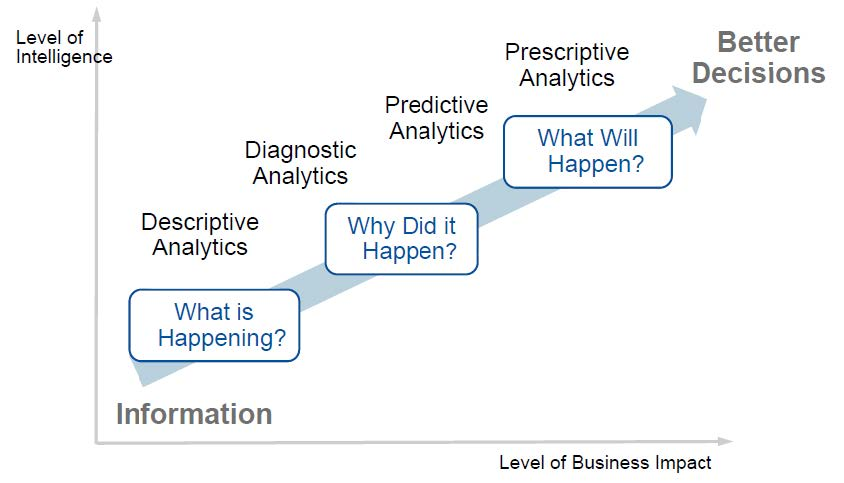
\includegraphics[width=\textwidth]{fig/analyseformen}
		\caption{Analyseformen von Big Data}
		\label{fig:analyseformen}
	\end{subfigure}
	~
	\begin{subfigure}[b]{0.4\textwidth}
		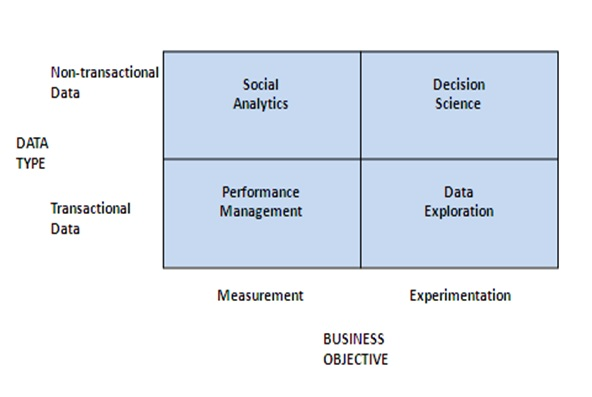
\includegraphics[width=\textwidth]{fig/strategy_bigdata}
		\caption{Strategien zum Einsatz von Big Data}
		\label{fig:strategy_bigdata}
	\end{subfigure}
\end{figure}
